\documentclass[
	letterpaper, % Paper size, specify a4paper (A4) or letterpaper (US letter)
	10pt, % Default font size, specify 10pt, 11pt or 12pt
]{CSUniSchoolLabReport}

%----------------------------------------------------------------------------------------
%	REPORT INFORMATION
%----------------------------------------------------------------------------------------

\title{Experiment Three\\ Fundamentals of Electromagnetics Lab \\ EECE2530/1} % Report title

\author{Michael \textsc{Brodskiy}\\ \small \href{mailto:Brodskiy.M@Northeastern.edu}{Brodskiy.M@Northeastern.edu}}

\date{October 18, 2023} % Date of the report

%----------------------------------------------------------------------------------------


\begin{document}

\maketitle % Insert the title, author and date using the information specified above

\begin{center}
	\begin{tabular}{l r}
		Date Performed: & October 11, 2023 \\ % Date the experiment was performed
        Partners: & Manas \textsc{Mahajan} \& Priyam \textsc{Modi} \\ % Partner names
		Instructor: & Professor \textsc{Marengo-Fuentes} \\ % Instructor/supervisor
        TAs: & Nicolas \textsc{Casilli} \& Farah \textsc{Ben Ayed} \\ % Teachers Assistants 
	\end{tabular}
\end{center}

\newpage

\begin{abstract}

The goal of this laboratory experiment was to determine the dielectric permittivity and resonance, $Q$, of different microstrip line resonators by measuring the transmission of the resonators. To do this, different microstrip lines were connected to the network analyzer, and the frequency and resonance index were measured, which was then used to calculate the dielectric permittivity.

\end{abstract}

\begin{flushleft}

  \textsc{Keywords:} \underline{Dielectric Permittivity}, \underline{Resonance}, \underline{Microstrip Line}, \underline{Energy Loss Mechanism}, \underline{Network Analyzer}, \underline{Frequency}, \underline{Resonance Index}

\end{flushleft}

\newpage

\section{Equipment}

\hspace{.5 in} Available equipment included:\\

\begin{itemize}

  \item Vector Network Analyzer (HP8714)

  \item Microwave Dielectric Circuit Boards:

    \begin{itemize}

      \item One Microstrip Line Resonator

      \item Four Microstrips Line Resonators

      \item Eight Microstrips Line Resonators

    \end{itemize}

  \item Type N to SMA connectors

  \item Coaxial Cables with SMA connectors

  \item Plexiglass Piece

\end{itemize}

\section{Pre-Lab}

\subsection{Question 1}

\begin{figure}[H]
  \centering
  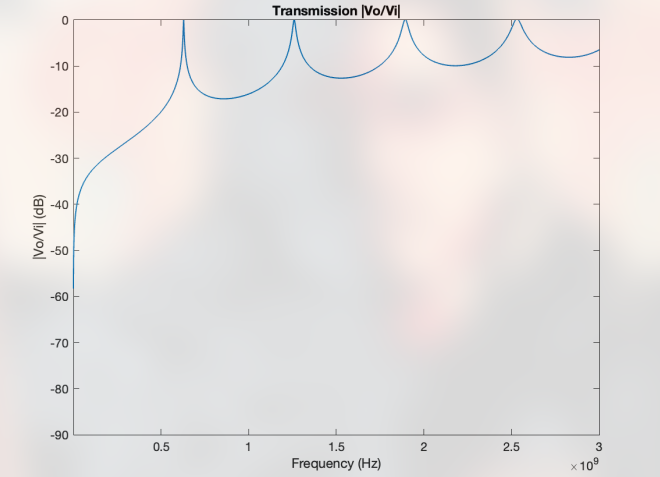
\includegraphics[width=.9\textwidth]{Figures/Lab Three/InitGraph.png}
  \caption{The Plot from the Given Code}
  \label{fig:1}
\end{figure}

\subsection{Question 2}

\begin{figure}[H]
  \centering
  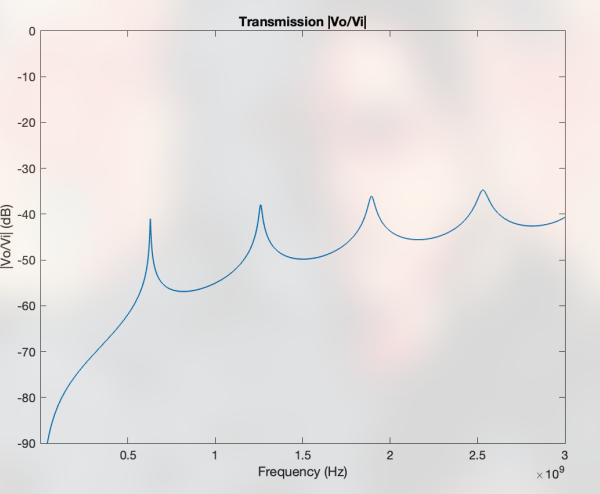
\includegraphics[width=.9\textwidth]{Figures/Lab Three/ModGraph.png}
  \caption{Graph from Modified Equation 7}
  \label{fig:2}
\end{figure}

After modifying equation 7, the plot changes to the one shown below, showing that the transmission never exceeds $0$[dB]. After including the reflection coefficient in the calculation, the peaks of $0$ reduced to peaks of around $-35$ to $-40$ [dB]. The peaks also have varying heights and do not all peak at $0$.

\begin{flushleft}
\textcolor{green}{\%Correction of Eq7}
\textsc{VoVi = @(x) (Eq7(x).*1).*(1+Rl1(x));} 
\end{flushleft}

\subsection{Question 3}

Figure \ref{fig:3} below shows traces for $C=5\cdot10^{-13}[\si{\farad}]$, $C=5\cdot10^{-12}[\si{\farad}]$ and $C=10\cdot10^{-12}[\si{\farad}]$

\begin{figure}[H]
  \centering
  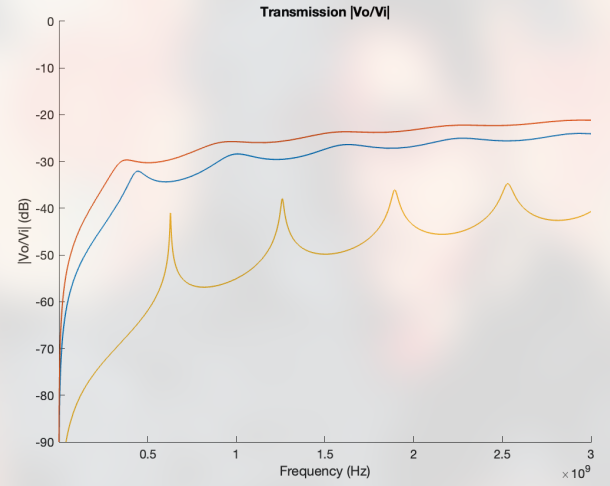
\includegraphics[width=.9\textwidth]{Figures/Lab Three/GraphTrio.png}
  \caption{Traces for 3 $C$ Values}
  \label{fig:3}
\end{figure}

For the first peaks, a higher capacitance value widens the FWHM. However, the value of the frequencies for which this zone occurs reduces in magnitude. Increasing the capacitance also increases the reflection because it creates an impedance mismatch which leads to a higher dB value on the $y$ axis. This corresponds to a larger reflected wave. Increasing the capacitance also reduces resonances.

\subsection{Question 4}

\begin{figure}[H]
  \centering
  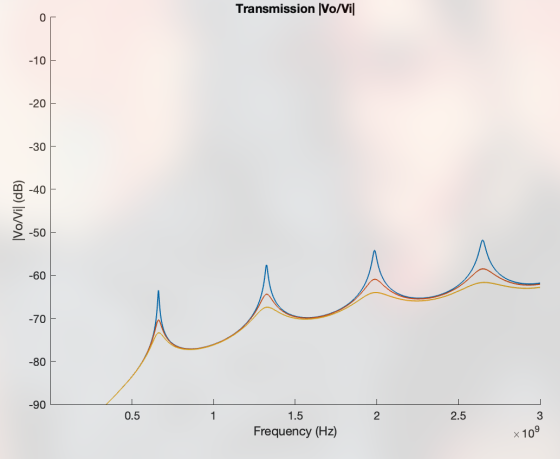
\includegraphics[width=.9\textwidth]{Figures/Lab Three/ThreePeaks.png}
  \caption{Question 4 Graph}
  \label{fig:4}
\end{figure}

Increasing the $\tan$ delta increases the FWHM and also decreases the value of the $y$-axis, showing that there are more reflections. This is expected, as introducing a loss tangent as a material property should cause more loss, and thus more reflections.

\section{Introduction \& Objectives}

We began this experiment by setting up the network analyzer to show the Smith Chart output of the microstrip lines for frequencies from $300[\si{\mega\hertz}]$ to $3[\si{\giga\hertz}]$. The impedance of the microstrip lines was observed and compared to the $50[\si{\ohm}]$ impedance of the network analyzer. 

	For each resonator, we measured the transmitted signal for three different resonators, taking note of the resonant frequencies, $f_o$ , and full width at half maximum, FWHM, for the first two resonance indexes of each. 

	A plexiglass piece was placed on top of the 4 microstrip parallel-plate resonator, and the resonant frequency and full width at half maximum were recalculated. The transmission was compared to that of the resonator without the plexiglass on top.

    The transmission of each resonator was compared to one another, and the measurements were used to calculate the dielectric permittivity, $\varepsilon_{eff}$ , and the resonance, $Q$ using the equations shown below. The dielectric permittivity and resonance were calculated separately for each of the three resonators and the transmission with the plexiglass.

    $$f_o=\frac{nc}{2d\sqrt{\varepsilon_{eff}}}\to\varepsilon_{eff}=\left( \frac{nc}{2df_o} \right)^2$$
    $$Q=\frac{f_o}{FWHM}=\frac{f_o}{\Delta f}$$

\section{Results \& Analysis} 

The results can be tabulated in the following manner:

\begin{center}
  \begin{tabular}[H]{|p{.15\textwidth}|p{.2\textwidth}|p{.2\textwidth}|p{.2\textwidth}|p{.2\textwidth}|}
    \hline
    & Resonant Frequency 1 ($f_{o,1}$) & FWHM 1 ($\Delta f$) & Resonant Frequency 2 ($f_{o,2}$) & FWHM 2 ($\Delta f$)\\
    \hline
    1 Microstrip & $544[\si{\mega\hertz}]$ & 451-655=204$[\si{\mega\hertz}]$ & $945[\si{\mega\hertz}]$ & $1100-804=206[\si{\mega\hertz}]$\\
    \hline
    4 Microstrip & $530[\si{\mega\hertz}]$ & 497-553=56$[\si{\mega\hertz}]$ & $2.23[\si{\giga\hertz}]$ & $2.238-2.221=17[\si{\mega\hertz}]$\\
    \hline
    4 Microstrip Parallel Plate & $2.067[\si{\giga\hertz}]$ & 2.134-2.036=98$[\si{\mega\hertz}]$ & N/A & N/A\\
    \hline
    4 Microstrip Parallel Plate with Plexiglass & $2.053[\si{\giga\hertz}]$ & 2.069-2.031=38$[\si{\mega\hertz}]$ & N/A & N/A\\
    \hline
  \end{tabular}
\end{center}

We then use the above obtained values, in tandem with given values:

$$\left\{\begin{array}{l}c=2.9979\cdot10^8\left[ \frac{\si{\meter}}{\si{\second}} \right]\\d=.089[\si{\meter}]\end{array}$$

  and the formulas from above, with $n$ as the resonant index, to get the following values:

  \begin{center}
    \begin{tabular}[H]{|c|c|c|c|c|}
     \hline
     & $\varepsilon_{eff,1}$ & $\varepsilon_{eff,2}$ & $Q_1$ & $Q_2$\\
     \hline
     1 Microstrip & 9.535 & 12.639 & 2.628 & 3.193\\
     \hline
     4 Microstrip & 10.045 & 2.23 & 9.464 & 131.176\\
     \hline
     4 Microstrip & .660 & — & 21.092 & —\\
     Parallel Plate & & & & \\
     \hline
     4 Microstrip & .669 & —  & 54.026 & — \\
     Parallel Plate & & & & \\
     w/Plexiglass & & & & \\
     \hline
    \end{tabular}
  \end{center}

\section{Conclusion}

\subsection{Questions}

\begin{enumerate}

  \item Using the Smith Chart output, discuss how well-matched the microstrip lines are to the $50[\si{\ohm}]$ impedance of the Network Analyzer.

    The microstrip lines were all well matched to the 50 ohm impedance of the network analyzer. The display showed concentric circles that slowly got smaller in radius until they terminated at the center point on the Smith chart, which indicates a scenario with matched impedance.

  \item How do the resonators differ from each other? Are the peaks the same?

    \begin{figure}[H]
      \centering
      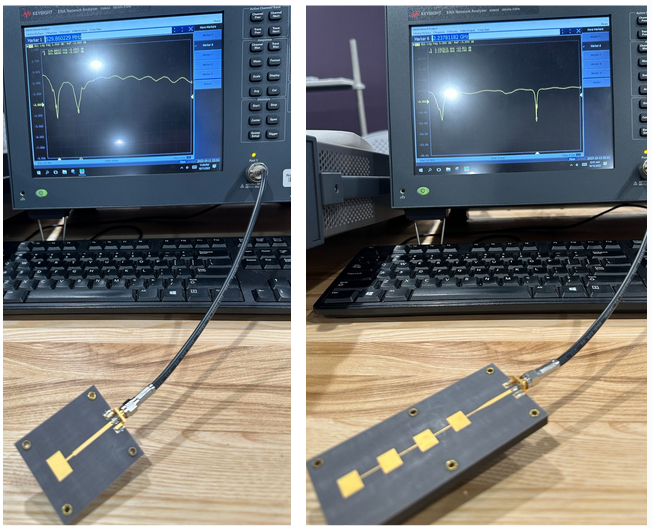
\includegraphics[width=.6\textwidth]{Figures/Lab Three/Peaks-1-4.png}
      \caption{1 and 4 Microstrip Lines}
      \label{fig:5}
    \end{figure}

    \begin{figure}[H]
      \centering
      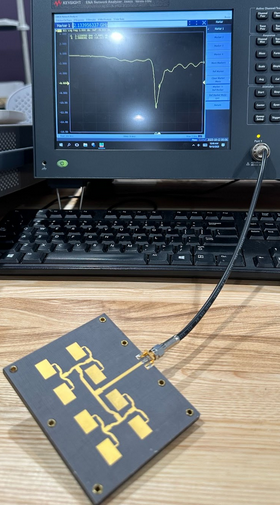
\includegraphics[width=.5\textwidth]{Figures/Lab Three/Peaks-4x2.png}
      \caption{4 Parallel Plate Microstrip Lines}
      \label{fig:6}
    \end{figure}

    As evident from figures \ref{fig:5} and \ref{fig:6}, all of the resonators differ in length and shape, causing the resonant frequencies to be different. The peaks are not the same as shown in the images above. The larger resonators have a larger wavelength due to the increase in the length of the transmission line.

  \item 

  \item Place a piece of plexiglass on top of one of the microstrip line resonators. How does the transmission change? How do you explain your result?

    As evident by figure \ref{fig:7}, placing plexiglass on top of the microstrip line resonator changes the dielectric constant of the microstrip structure, causing the transmission characteristics to change. The transmission changes by resonating at a lower frequency and at a smaller half-power bandwidth. This is likely due to the added loss from adding a dielectric.

    \begin{figure}[H]
      \centering
      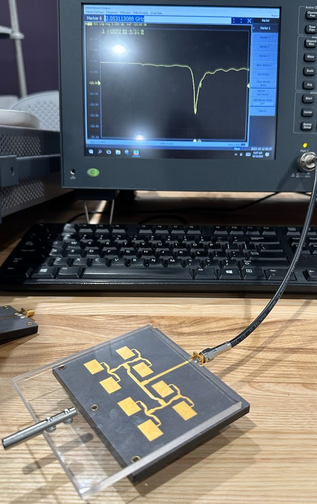
\includegraphics[width=.6\textwidth]{Figures/Lab Three/Peaks-Plex.png}
      \caption{Plexiglass Peaks}
      \label{fig:7}
    \end{figure}

  \item The resonators have different gaps. Is there any systematic change in the $Q$ as a function of gap size?

As the number of resonators increased, the gap size decreased. This led to a higher experimental $Q$ value as shown in the results chart for each resonator. 

\item If the resonance $Q$ does not change much between the resonators, what would you conclude about the relative importance of the two sources of energy loss in the resonators (dielectric and ohmic)? Can you estimate what the dielectric loss tangent is, assuming that ohmic losses are small compared to the dielectric?

If the resonance $Q$ does not change much between the resonators, we could conclude that the relative importance of dielectric and ohmic sources of energy loss in resonators is about the same in all resonators. The energy loss would be pretty consistent between the different resonators, indicating the dielectric properties of the resonators’ conducting materials are similar. We estimate the dielectric loss tangent to be around 0.02.

\end{enumerate}

\subsection{Summary}

In this lab, we learned how to find the effective permittivity using the relative permittivity and characteristics of a transmission line. Using the Vector Network Analyzer (VNA), we found the resonant frequency of each of 3 microstrip resonators. We then proceeded to find the half power bandwidth at the $-3$[dB] level from the peak, and used the observed values to calculate the effective permittivity of the various resonators. We also calculated the Q factor, which defines the shape of the resonance curve, for all 3 resonators and their resonant frequencies in the range of $300[\si{\mega\hertz}]$ to $3[\si{\giga\hertz}]$. This experiment allowed us to see firsthand the effect that different shapes and layouts of microstrips can have on the effective permittivity, $Q$ factor, and resonant frequency, as is evident from the results we found above.

\end{document}
